% ============================================================================
%  The Polyglot's Shorthand -- Version 1.2 Architecture and Interim Results
%  Compile:  pdflatex v12_architecture && pdflatex v12_architecture   (or: latexmk -pdf)
%  Engine:   pdfLaTeX (emoji are written as named placeholders, see \emo)
%  Status:   all phases complete (teachers, student, export, latency).
%  Every number is taken from v12/results/*.json.
% ============================================================================
\documentclass[11pt,a4paper]{article}

% ---------------------------------------------------------------- packages --
\usepackage[T1]{fontenc}
\usepackage[utf8]{inputenc}
\usepackage{lmodern}
\usepackage[margin=2.3cm]{geometry}
\usepackage{microtype}
\usepackage{amsmath,amssymb,amsthm,bm}
\usepackage{booktabs,tabularx,multirow}
\usepackage[table]{xcolor}
\usepackage{graphicx}
\usepackage{tikz}
\usetikzlibrary{arrows.meta,positioning,fit,calc,backgrounds}
\usepackage{pgfplots}
\pgfplotsset{compat=1.17}
\usepackage{algorithm}
\usepackage[noend]{algpseudocode}
\usepackage{caption}
\usepackage{enumitem}
\usepackage{listings}
\usepackage[colorlinks=true,linkcolor=accent,citecolor=accent,urlcolor=accent]{hyperref}
\usepackage[nameinlink,capitalise]{cleveref}

% ------------------------------------------------------------------ styling --
\definecolor{accent}{RGB}{31,78,121}
\definecolor{accentlight}{RGB}{214,228,240}
\definecolor{warn}{RGB}{176,58,46}
\definecolor{okgreen}{RGB}{39,119,72}
\definecolor{muted}{RGB}{110,110,110}
\definecolor{pending}{RGB}{190,120,0}
\captionsetup{font=small,labelfont={bf,color=accent}}
\setlist{nosep,leftmargin=1.4em}
\lstset{basicstyle=\ttfamily\small,columns=fullflexible,frame=single,
        rulecolor=\color{muted!40},backgroundcolor=\color{accentlight!35},
        xleftmargin=0.5em,xrightmargin=0.5em,breaklines=true}

\newtheorem{definition}{Definition}
\newtheorem{proposition}{Proposition}
\theoremstyle{remark}
\newtheorem*{remark}{Remark}

% ------------------------------------------------------------------- macros --
\newcommand{\lbl}[1]{\texttt{#1}}
\newcommand{\hi}[1]{\textit{#1}}
\newcommand{\emo}[1]{\textsf{\small$\langle$#1$\rangle$}}
\newcommand{\R}{\mathbb{R}}
\newcommand{\x}{\bm{x}}
\newcommand{\W}{\bm{W}}
\newcommand{\bb}{\bm{b}}
\newcommand{\z}{\bm{z}}
\newcommand{\p}{\bm{p}}
\newcommand{\pend}{\textcolor{pending}{\textbf{pending}}}
\newcommand{\nr}{\textcolor{muted}{not run}}
\DeclareMathOperator*{\argmin}{arg\,min}
\DeclareMathOperator*{\argmax}{arg\,max}
\DeclareMathOperator{\softmax}{softmax}
\DeclareMathOperator{\CE}{CE}
\DeclareMathOperator{\KL}{KL}
\DeclareMathOperator{\LN}{LN}
\DeclareMathOperator{\GELU}{GELU}
\newcommand{\cm}[2]{\cellcolor{accent!#1}\ifnum#1>45\color{white}\fi#2}

% ----------------------------------------------------------------- metadata --
\title{\vspace{-1.2em}\textbf{The Polyglot's Shorthand --- Version 1.2}\\[0.3em]
  \large Distilling a Pretrained Hinglish Encoder into a Hashed-Piece Transformer\\[0.4em]
  \normalsize\color{muted}Architecture, Protocol and Results (compared with v1.1)}
\author{Harsh Raj}
\date{September 2026}

% ============================================================================
\begin{document}
\maketitle

\begin{abstract}
\noindent
Version~1.1 (a 827K-parameter NumPy model: hashed linear branch plus one
self-attention layer) reached intent macro-F1 $0.901$ $[0.782, 0.970]$ and
sentiment macro-F1 $0.845$ $[0.718, 0.944]$ on a 190-row, 44-group development
test, but left four documented failures: unseen affect words, a spurious
\hi{nahi}$\Rightarrow$\lbl{negative} cue, negation scope and keyword-driven
intent routing. Version~1.2 separates two hypotheses---\emph{pretrained
knowledge} and \emph{more diverse data}---and then distils the result into a
deployable student. A pretrained Hinglish encoder
(\lbl{l3cube-pune/hing-roberta-mixed}, 278M parameters) trained on the v1.1
split alone fixes sentiment (paired $\Delta = +0.159$ $[+0.056, +0.282]$) but
not intent ($+0.032$ $[-0.061, +0.142]$). Trained additionally on 1{,}202
generated support messages, 2{,}323 augmented variants and 4{,}000 public
sentiment tweets, the same encoder (teacher~v2) reaches intent $0.966$
$[0.92, 0.99]$ (paired $+0.071$ $[-0.007, +0.172]$), raises negation-scope
intent accuracy on a new hand-written contrast set from $0.65$ to $0.90$ and
solves 29 of 40 contrast pairs (v1.1: 10). Its soft labels on 66{,}166
sentences are distilled into an 11.88M-parameter student that keeps v1.1's
hashed word/alias/character-$n$-gram pieces, adds four pre-LN transformer
blocks and retains the residual hashed linear branch; it is deployed without
PyTorch (NumPy + ONNX Runtime, INT8; p95 0.81\,ms on test messages and
4.29\,ms at 512 code points on an Apple M2 with two threads). The student does
\emph{not} keep the teacher's gains: intent $0.914$ $[0.81, 0.98]$ and
sentiment $0.911$ $[0.82, 0.98]$ are not resolved against v1.1, sentiment is
significantly below teacher~v2 ($-0.092$ $[-0.184, -0.020]$) and varies across
seeds (sd $0.049$), knowledge distillation is not shown to help over a no-KD
student, and removing the hashed linear branch appears to improve intent
($0.958$). INT8 quantization is lossless on these sets. All evaluation data
remain LLM-generated, so gains may partly reflect the generator's style.
\end{abstract}

\tableofcontents
\vspace{1em}\hrule

% ============================================================================
\section{From v1.1 to v1.2}
\label{sec:overview}

\begin{table}[h]
\centering\small
\caption{Version lineage. v1.2 keeps the v1.1 hashing byte-for-byte and adds a teacher, new data and a larger, deployable student.}
\label{tab:lineage}
\begin{tabularx}{\linewidth}{@{}l X X X@{}}
\toprule
& v1.0 & v1.1 & v1.2 \\
\midrule
Model & Hashed sparse linear, 2 heads & v1.0 linear $+$ 1 self-attention layer ($d{=}32$) & Teacher (XLM-R base) $\to$ student: hashed pieces $+$ 4 pre-LN blocks ($d{=}256$) $+$ v1.0 linear branch \\
Parameters & 294{,}921 & 827{,}721 & teacher 278{,}050{,}569; student 11{,}878{,}419 \\
Training data & 120 rows & 536 rows (213 seeds) & 536 $+$ 1{,}202 generated $+$ 2{,}323 augmented $+$ public tweets (sentiment) $+$ 50k unlabeled (KD) \\
Framework & NumPy & NumPy, hand-derived gradients & PyTorch on free Colab T4; deployment NumPy $+$ ONNX Runtime \\
Evaluation splits & v1.0 split & regenerated v1.1 split & \textbf{exact v1.1 split} (digest-checked) $+$ contrast set \\
\bottomrule
\end{tabularx}
\end{table}

\paragraph{Research questions.}
\begin{enumerate}
  \item[\textbf{Q1}] Does pretrained Hinglish knowledge alone fix the v1.1 failures? (\cref{sec:teacher1})
  \item[\textbf{Q2}] Does more diverse, targeted data help beyond pretraining? (\cref{sec:teacher2}, data ablation)
  \item[\textbf{Q3}] Does a student under 15M parameters and 5\,ms keep the teacher's gains? (\cref{sec:student,sec:results})
\end{enumerate}

\begin{figure}[t]
\centering
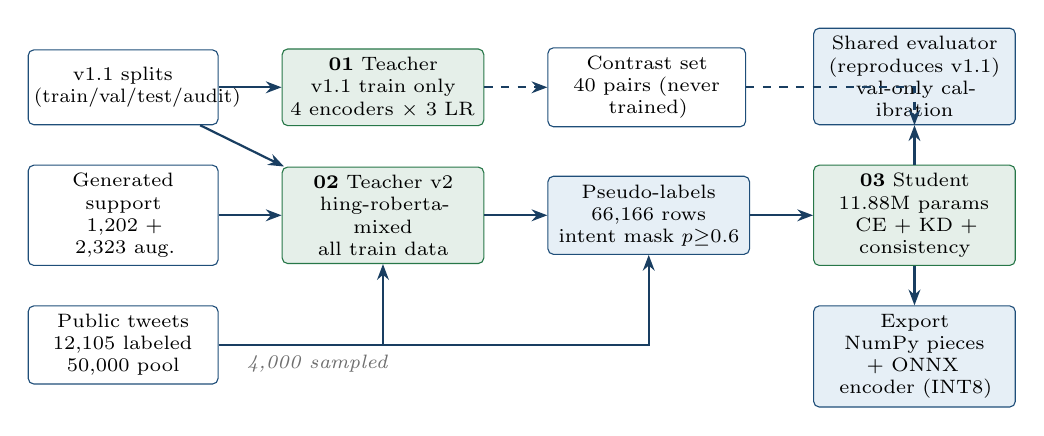
\begin{tikzpicture}[
  node distance=0.5cm and 0.45cm,
  box/.style={draw=accent,rounded corners=2pt,fill=accentlight!60,minimum height=0.95cm,align=center,font=\scriptsize,inner sep=3pt,text width=2.35cm},
  dat/.style={box,fill=white,text width=2.2cm},
  gpu/.style={box,fill=okgreen!12,draw=okgreen},
  arr/.style={-{Stealth[length=2mm]},thick,accent!80!black},
  lab/.style={font=\scriptsize\itshape,text=muted}]
  \node[dat] (v11) {v1.1 splits\\(train/val/test/audit)};
  \node[dat,below=of v11] (gen) {Generated support\\1{,}202 $+$ 2{,}323 aug.};
  \node[dat,below=of gen] (pub) {Public tweets\\12{,}105 labeled\\50{,}000 pool};
  \node[gpu,right=0.8cm of v11] (t1) {\textbf{01} Teacher\\v1.1 train only\\4 encoders $\times$ 3 LR};
  \node[gpu,right=0.8cm of gen] (t2) {\textbf{02} Teacher v2\\hing-roberta-mixed\\all train data};
  \node[box,right=0.8cm of t2] (kd) {Pseudo-labels\\66{,}166 rows\\intent mask $p{\ge}0.6$};
  \node[gpu,right=0.8cm of kd] (st) {\textbf{03} Student\\11.88M params\\CE $+$ KD $+$ consistency};
  \node[box,below=of st] (onnx) {Export\\NumPy pieces $+$ ONNX\\encoder (INT8)};
  \node[box,above=of st] (eval) {Shared evaluator\\(reproduces v1.1)\\val-only calibration};
  \node[dat,right=0.8cm of t1,text width=2.3cm] (con) {Contrast set\\40 pairs (never trained)};
  \draw[arr] (v11) -- (t1);
  \draw[arr] (v11) -- (t2);
  \draw[arr] (gen) -- (t2);
  \draw[arr] (pub) -| node[lab,pos=0.3,below]{4{,}000 sampled} (t2);
  \draw[arr] (t2) -- (kd);
  \draw[arr] (kd) -- (st);
  \draw[arr] (pub.east) -| (kd.south);
  \draw[arr] (st) -- (onnx);
  \draw[arr] (st) -- (eval);
  \draw[arr,dashed] (t1) -- (con);
  \draw[arr,dashed] (con) -| (eval);
\end{tikzpicture}
\caption{v1.2 pipeline. Green boxes run on a free Colab T4 as self-contained, auto-resuming notebooks; everything else runs on the Mac. Test, audit and contrast are only ever scored.}
\label{fig:pipeline}
\end{figure}

% ============================================================================
\section{Protocol and Invariants}
\label{sec:protocol}

\begin{enumerate}
  \item \textbf{Exact v1.1 splits.} Train/validation/test/audit and group ids are exported from the files whose SHA-256 digests are recorded in the v1.1 \texttt{results.json}; nothing is regenerated or reshuffled. A \texttt{test\_stress} copy applies the unchanged 14-entry stress map.
  \item \textbf{Validation only for choices.} Early stopping, model/learning-rate selection, temperature and review threshold use validation NLL/accuracy only. Test, audit and contrast are written by notebooks and read only by the evaluator.
  \item \textbf{All new data to TRAIN, filtered.} A new message is dropped if its character-3-gram Jaccard similarity to any validation, test, audit or contrast message exceeds $0.6$:
  \begin{equation}
    J(a,b) = \frac{|G_3(a)\cap G_3(b)|}{|G_3(a)\cup G_3(b)|},\qquad G_3(s)=\{\text{3-grams of } \texttt{"\ "}\,\nu(s)\,\texttt{"\ "}\}.
  \end{equation}
  An inverted index returns exact $|G_3(a)\cap G_3(b)|$ and matches brute force on all 616 checked queries.
  \item \textbf{Identical evaluator.} One evaluator scores every system from saved logits; it reproduces every v1.1 whitepaper test number (macro-F1 and CIs, ECE, coverage, stress, emoji pairs, audit).
  \item \textbf{Uncertainty.} Macro-F1 intervals: 5{,}000 resamples of the 44 test groups (seed 0); paired differences on identical resamples.
  \item \textbf{Hash parity.} The v1.1 hashing is copied into the bundle and checked against 50 stored fixtures (indices exact, values within $10^{-6}$) plus a digest over all 1{,}148 exported rows: identical under Python 3.10, 3.12, 3.13 (Colab) and 3.14, i.e.\ Unicode 13.0--16.0.
\end{enumerate}

% ============================================================================
\section{Data}
\label{sec:data}

\subsection{Reused v1.1 Splits}
\begin{table}[h]
\centering\small
\caption{Evaluation and base training data (unchanged from v1.1).}
\label{tab:splits}
\begin{tabular}{@{}lrrcl@{}}
\toprule
Split & Rows & Groups & Neg / Neu / Pos & Use \\
\midrule
Train       & 536 & 130 & 187 / 181 / 168 & training \\
Validation  & 158 &  39 & \phantom{0}50 / \phantom{0}58 / \phantom{0}50 & selection, early stopping, calibration \\
Test        & 190 &  44 & \phantom{0}64 / \phantom{0}65 / \phantom{0}61 & development test (report only) \\
Test-stress & 190 &  44 & same & unseen misspellings (report only) \\
Audit       &  24 &  24 & \phantom{00}7 / \phantom{0}15 / \phantom{00}2 & frozen audit (report only) \\
\bottomrule
\end{tabular}
\end{table}

\subsection{Public Hinglish Data (out of domain)}
\begin{table}[h]
\centering\small
\caption{Public sources after cleaning (Latin script only, 3--60 words, $\ge2$ Romanized Hindi function words, mojibake repair, mention/URL removal, exact de-duplication). Near-duplicates of protected messages removed: \textbf{0}.}
\label{tab:public}
\begin{tabularx}{\linewidth}{@{}l l r r X@{}}
\toprule
Source & License & Raw & Kept & Use \\
\midrule
SemEval-2020 T9 SentiMix (HF \texttt{RTT1/SentiMix}) & research-use Twitter & 20{,}000 & 12{,}080 & labeled sentiment, intent masked \\
Code-mixed tweets (HF \texttt{Abhishek4896/...}) & MIT & 498 & 25 & labeled sentiment \\
PHINC (HF \texttt{LingoIITGN/PHINC}) & CC-BY-4.0 & 13{,}738 & 9{,}561 & unlabeled pool (8{,}000) \\
L3Cube-HingLID (GitHub) & CC-BY-NC-SA-4.0 & 44{,}455 & 42{,}543 & unlabeled pool (35{,}957) \\
CMU Hinglish DoG (HF \texttt{festvox/...}) & CC-BY-SA-3.0 & 9{,}962 & 7{,}146 & unlabeled pool (6{,}043) \\
\bottomrule
\end{tabularx}
\end{table}
Rejected: a 100k ``code-mixed sentiment'' set that is machine-translated Devanagari/Bengali/English reviews (not Romanized), and the multi-GB HingCorpus file (HingLID from the same L3Cube Twitter source used instead). No public Hinglish customer-support intent data was found.

\subsection{Generated Support Data and Augmentation}
1{,}202 messages in 591 paraphrase families (short of the planned $\sim$1{,}500), written in three batches with seven personas, 2--36 words (mean 11.3), 10.4\% with emoji, regional spellings (\hi{kaiku, apun, kithe, kado}), formal Hindi and heavy shorthand. Rows are tagged by targeted phenomenon (\cref{tab:gen}). One near-duplicate was removed. A self-audit corrected two labels.

\begin{table}[h]
\centering\small
\caption{Generated data: label distribution (left) and targeted phenomena (right).}
\label{tab:gen}
\begin{tabular}{@{}lccc@{}}
\toprule
Intent & Neg & Neu & Pos \\
\midrule
\lbl{cancel\_order}  & 65 & 127 & 56 \\
\lbl{refund}         & 62 & 98 & 54 \\
\lbl{track\_order}   & 59 & 97 & 48 \\
\lbl{not\_received}  & 54 & 84 & 42 \\
\lbl{damaged\_item}  & 50 & 80 & 42 \\
\lbl{feedback}       & 61 & 57 & 66 \\
\midrule
Total (1{,}202)      & 351 & 543 & 308 \\
\bottomrule
\end{tabular}
\hspace{1.2em}
\begin{tabular}{@{}lr@{}}
\toprule
Tag & Rows \\
\midrule
negation scope & 97 \\
neutral with \hi{nahi} & 119 \\
negated negative & 99 \\
varied affect word & 151 \\
praise then request & 82 \\
mixed intent (main request) & 66 \\
\bottomrule
\end{tabular}
\end{table}

\emph{Augmentation.} Each v1.1-train or generated row yields up to two variants: a \emph{map} variant (v1.1 shorthand and respelling maps, applied per token with $p{=}0.6$) and a \emph{noise} variant (vowel drop, QWERTY-neighbour swap, elongation, transposition; per editable token with $p{=}0.3$). Negators (\hi{nahi, mat, bina, koi, na, not}, \dots), emoji, punctuation and numbers are never edited, token counts never change, and a variant is rejected if it introduces any stress-map output (\hi{nahii, karr, hey, orrder, refnd}, \dots). Result: 2{,}323 variants (786 map, 1{,}537 noise), 2 near-duplicates removed. An automated check over 17{,}680 noisy variants of all v1.1 texts found zero stress outputs and zero edited protected tokens.

\subsection{Diagnostic Contrast Set}
40 hand-written minimal pairs (80 messages), written in Phase~0 before any generated data and never used for any choice: 10 pairs each for \emph{negation scope} (a negated action is not the request), \emph{neutral nahi}, \emph{negated negative} and \emph{unseen affect}. Maximum Jaccard to any v1.1 message: 0.37.

\paragraph{Overlap risk.} 18 of the 32 affect words in the contrast set (\hi{pareshan, tang, dukhi, nirash, raahat, sukoon, chinta, prasann}, \dots) enter training only through the generated data, and generated vocabulary raises coverage of validation/test vocabulary from 0.687/0.701 to 0.949/0.944. After Phase~2, \emph{unseen affect} measures learning from generated data, not generalisation.

% ============================================================================
\section{Teacher}
\label{sec:teacher}

\subsection{Model}
For a message $s$, a pretrained encoder $f_\phi$ produces contextual subword states $\bm h_{1:n}$; masked mean pooling and two linear heads give
\begin{equation}
  \bar{\bm h} = \frac{\sum_{i} m_i \bm h_i}{\sum_i m_i},\qquad
  \z^{I} = \W_I\,\mathrm{Drop}(\bar{\bm h}) + \bb_I \in\R^{6},\qquad
  \z^{S} = \W_S\,\mathrm{Drop}(\bar{\bm h}) + \bb_S \in\R^{3}.
\end{equation}
The loss is the v1.1 class-balanced cross-entropy with per-row head masks $\mu^k_i\in\{0,1\}$ (public sentiment rows have $\mu^I_i=0$):
\begin{equation}
  \mathcal{L} = \sum_{k\in\{I,S\}} \frac{1}{\sum_i\mu^k_i}\sum_i \mu^k_i\,\alpha^k_{y^k_i}\,\CE\big(\softmax(\z^k_i), y^k_i\big),
  \qquad \alpha^k_c = \frac{N_k}{K_k\max(n^k_c,1)} .
\end{equation}
Optimization: AdamW (weight decay 0.01, none on biases/LayerNorm), linear warm-up then linear decay, gradient clipping at 1.0, fp16 autocast with dynamic loss scaling, early stopping on the unweighted validation NLL of both heads (the v1.1 definition).

\begin{algorithm}[h]
\caption{Resumable run on a free GPU (one encoder, one learning rate)}
\label{alg:resume}
\small
\begin{algorithmic}[1]
\If{\texttt{status.json} says done} \State \Return \Comment{Run all again after a disconnect}\EndIf
\State load encoder; build optimizer, scheduler, scaler
\If{\texttt{last.pt} exists} \State restore weights (fp16), scheduler, RNG, best NLL, patience counter, history \EndIf
\For{epoch $e$ from resumed epoch to $E$}
  \State shuffle with generator seeded by $1000\cdot\text{seed}+e$ \Comment{identical order after resume}
  \State train; compute validation NLL; if improved write \texttt{best.pt}
  \State atomically write \texttt{last.pt} (temp file $+$ rename) to Google Drive
  \If{patience exhausted} \textbf{break} \EndIf
\EndFor
\State load \texttt{best.pt}; write logits for every predict file; mark done; delete checkpoints
\end{algorithmic}
\end{algorithm}

\subsection{Q1: Pretraining Only (v1.1 train split)}
\label{sec:teacher1}
\begin{table}[h]
\centering\small
\caption{Twelve teacher runs on the v1.1 train split (Colab T4, 38 min total). Selection by validation NLL only; test columns are listed for transparency and were not used.}
\label{tab:teacher1}
\setlength{\tabcolsep}{4pt}
\begin{tabular}{@{}l c c c c c c@{}}
\toprule
Run & Val.\ NLL & Test intent F1 & Test sent.\ F1 & Emoji pairs & Audit err. & Contrast both-correct \\
\midrule
hing-roberta, 2e-5          & 0.132 & .955 & 1.000 & 12/12 & 3 & .750 \\
hing-roberta, 3e-5          & 0.094 & .954 & 1.000 & 12/12 & 1 & .762 \\
hing-roberta, 5e-5          & 0.101 & .951 & 1.000 & 12/12 & 1 & .738 \\
hing-roberta-mixed, 2e-5    & 0.114 & .955 & 1.000 & 12/12 & 1 & .713 \\
hing-roberta-mixed, 3e-5    & 0.085 & .951 & 1.000 & 12/12 & 1 & .725 \\
\textbf{hing-roberta-mixed, 5e-5} & \textbf{0.080} & \textbf{.929} & \textbf{1.000} & \textbf{12/12} & \textbf{1} & \textbf{.738} \\
hing-bert, 2e-5             & 0.260 & .871 & .861 & 3/12 & 2 & .425 \\
hing-bert, 3e-5             & 0.253 & .903 & .896 & 9/12 & 2 & .475 \\
hing-bert, 5e-5             & 0.269 & .891 & .882 & 6/12 & 2 & .475 \\
muril-base-cased, 2e-5      & 1.296 & .863 & .791 & 0/12 & 3 & .500 \\
muril-base-cased, 3e-5      & 1.238 & .934 & .822 & 0/12 & 3 & .575 \\
muril-base-cased, 5e-5      & 1.143 & .923 & .828 & 0/12 & 4 & .475 \\
\bottomrule
\end{tabular}
\end{table}

\paragraph{Emoji visibility.} The BERT-vocabulary tokenizers (hing-bert, MuRIL) map every emoji in all 261 emoji-bearing messages to \texttt{[UNK]}; the XLM-R tokenizers keep them. This alone explains the 0--9/12 emoji-pair results. The selected run is the one with the lowest validation NLL, even though it is not the best on test intent: selection never looks at test.

\paragraph{Verdict.} Pretraining fixes sentiment on every set (test F1 $1.000$; positive recall $1.00$; contrast sentiment accuracy 0.96 average vs 0.70) but not intent ($+0.032$ $[-0.061, +0.142]$), is \emph{less} stable than v1.1 under unseen misspellings (consistency 92.6\% vs 97.4\%), and still routes \hi{cancel mat karna sirf order track karke batao} to \lbl{cancel\_order}. The perfect sentiment score is a ceiling: validation sentiment accuracy is 0.943 and no test message has Jaccard $>0.6$ to any training message.

\subsection{Q2: Teacher v2 (pretraining $+$ new data)}
\label{sec:teacher2}
Same encoder and selection rule, trained on 8{,}061 rows (v1.1 train 536, generated 1{,}202, augmented 2{,}323, and a fixed seeded sample of 4{,}000 public tweets with the intent loss masked), batch 32, $\le$6 epochs, patience 2, two learning rates, 10.2 min on a T4. Both runs peaked at epoch 2 (validation NLL 0.0528 at 3e-5; \textbf{0.0472} at 5e-5, selected). The 3e-5 run scored higher on the contrast set (0.863 vs 0.825) and stress intent (0.955 vs 0.933); it was not selected because selection uses validation only.

\begin{table}[h]
\centering\small
\caption{Row-normalized test intent confusion matrices (counts; shading $\propto$ row share). Rows are true labels.}
\label{tab:cm}
\setlength{\tabcolsep}{4pt}
\begin{tabular}{@{}l cccccc c cccccc@{}}
\toprule
& \multicolumn{6}{c}{\textbf{v1.1}} && \multicolumn{6}{c}{\textbf{Teacher v2}}\\
\cmidrule(lr){2-7}\cmidrule(lr){9-14}
True & can & ref & trk & nrc & dmg & fb && can & ref & trk & nrc & dmg & fb \\
\midrule
\lbl{cancel}   & \cm{60}{36} & 0 & 0 & 0 & 0 & 0 && \cm{60}{36} & 0 & 0 & 0 & 0 & 0 \\
\lbl{refund}   & \cm{9}{3} & \cm{51}{17} & 0 & 0 & 0 & 0 && \cm{3}{1} & \cm{57}{19} & 0 & 0 & 0 & 0 \\
\lbl{track}    & 0 & 0 & \cm{58}{30} & \cm{2}{1} & 0 & 0 && 0 & 0 & \cm{52}{27} & \cm{2}{1} & 0 & \cm{6}{3} \\
\lbl{not\_rcv} & 0 & 0 & 0 & \cm{48}{21} & 0 & \cm{12}{5} && 0 & 0 & 0 & \cm{60}{26} & 0 & 0 \\
\lbl{damaged}  & 0 & 0 & 0 & 0 & \cm{43}{15} & \cm{17}{6} && 0 & 0 & 0 & 0 & \cm{60}{21} & 0 \\
\lbl{feedback} & 0 & 0 & \cm{3}{3} & 0 & 0 & \cm{57}{53} && 0 & 0 & \cm{2}{2} & 0 & 0 & \cm{58}{54} \\
\bottomrule
\end{tabular}
\end{table}

\begin{table}[h]
\centering\small
\caption{Contrast set per phenomenon: intent accuracy / sentiment accuracy (rows) and pairs with both members fully correct. NS negation scope, NN neutral \hi{nahi}, NG negated negative, UA unseen affect ($^\dagger$ affect words present in generated training data).}
\label{tab:contrast}
\begin{tabular}{@{}l cc cc cc cc c@{}}
\toprule
& \multicolumn{2}{c}{NS} & \multicolumn{2}{c}{NN} & \multicolumn{2}{c}{NG} & \multicolumn{2}{c}{UA$^\dagger$} & Pairs \\
\cmidrule(lr){2-3}\cmidrule(lr){4-5}\cmidrule(lr){6-7}\cmidrule(lr){8-9}
System & int & sent & int & sent & int & sent & int & sent & (of 40) \\
\midrule
v1.1                 & .65 & .90 & .85 & .75 & .90 & .45 & .85 & .70 & 10 \\
Teacher (v1.1 data)  & .70 & .95 & .80 & 1.00 & .70 & 1.00 & .90 & .90 & 24 \\
Teacher v2           & \textbf{.90} & .90 & \textbf{.90} & .95 & .70 & 1.00 & .95 & 1.00 & \textbf{29} \\
Student $+$ KD (s42) & .80 & .85 & .90 & .85 & .75 & .65 & .85 & .85 & 17 \\
Student no-KD (s42)  & .70 & .85 & .90 & .85 & .80 & .65 & .80 & .95 & 18 \\
Student $+$ KD w/o linear & .85 & .85 & .90 & .90 & .65 & .70 & .85 & .95 & 20 \\
\bottomrule
\end{tabular}
\end{table}

\paragraph{Reading the teachers.} New data moves negation-scope intent accuracy from 0.70 to 0.90 and fixes the long-standing audit error, while feedback$\to$operational and \lbl{not\_received}$\to$\lbl{feedback} confusions largely disappear (\cref{tab:cm}). On the test split the data effect over the Phase~1 teacher is \emph{not} resolved: intent $+0.040$ $[-0.028, +0.121]$, $P(\Delta>0)=0.85$; sentiment is at the ceiling for both. Remaining errors are keyword-driven: \hi{otp nahi mila} and complaints about delays are routed to \lbl{not\_received}, and feedback about packing or delivery to operational intents.

\subsection{Pseudo-labels for Distillation}
For every sentence $s$ the selected teacher~v2 provides logits $(\z^{I}_{\text{T}}, \z^{S}_{\text{T}})$. The intent-KD mask is
\begin{equation}
  \kappa^I(s) = \mathbb{1}[s \in \text{support data}]\cdot\mathbb{1}\big[\max_c \softmax(\z^I_{\text{T}}(s))_c \ge 0.6\big],\qquad
  \kappa^S(s) = 1 .
\end{equation}
\begin{table}[h]
\centering\small
\caption{Pseudo-label statistics (\texttt{results/kd\_stats.json}).}
\label{tab:kd}
\begin{tabular}{@{}l r c c c@{}}
\toprule
KD set & Rows & Teacher = gold (intent) & Teacher = gold (sentiment) & Intent KD kept \\
\midrule
v1.1 train      & 536    & 1.000 & 1.000 & 1.000 \\
Generated       & 1{,}202 & 0.997 & 0.994 & 0.997 \\
Augmented       & 2{,}323 & 1.000 & 0.997 & 0.997 \\
Public labeled  & 12{,}105 & -- & 0.710 & 0 (masked) \\
Unlabeled pool  & 50{,}000 & -- & -- & 0 (masked) \\
\bottomrule
\end{tabular}
\end{table}
On support rows the teacher reproduces the gold labels it was trained on, so KD there mainly transfers the \emph{shape} of the distribution (softened at $T=2$). The new information is on the 62{,}105 public sentences (teacher sentiment distribution on the pool: 22{,}902 neutral, 15{,}189 negative, 11{,}909 positive).

% ============================================================================
\section{Student Architecture}
\label{sec:student}

\subsection{Input: v1.1 Hashed Pieces, Unchanged}
Let $\nu$ be the v1.1 normalizer and $t_{1:T}$ the tokens of $\nu(s)$ (pattern \verb!\w+|[^\w\s]!, $T\le T_{\max}=128$). Each token $t_i$ yields the piece set
\begin{equation}
  \mathcal{B}_i = \Big\{h_B(\texttt{tw:}t_i),\; h_B(\texttt{ta:}\mathrm{alias}(t_i))\Big\}\cup\Big\{h_B(\texttt{tc}n\texttt{:}g) : g \in \text{$n$-grams of } \texttt{<}t_i\texttt{>},\ n\in\{3,4\}\Big\},
\end{equation}
with $h_B(f)=\mathrm{CRC32}(\mathrm{UTF8}(f)) \bmod B$. v1.2 uses $B = 2^{15}$ (v1.1: $2^{14}$); the key strings are identical, so the v1.1 hash fixtures test both.

\subsection{Encoder}
\begin{align}
  \bm X_i &= \frac{1}{|\mathcal{B}_i|}\sum_{j\in\mathcal{B}_i}\bm E_j + \bm P_i, && \bm E\in\R^{B\times d},\ \bm P\in\R^{T_{\max}\times d}\quad\text{(\texttt{EmbeddingBag}, mean)} \label{eq:embed}\\
  \bm U^{(\ell)} &= \bm X^{(\ell-1)} + \mathrm{MHA}\big(\LN(\bm X^{(\ell-1)})\big), && \ell = 1,\dots,4 \\
  \bm X^{(\ell)} &= \bm U^{(\ell)} + \bm W_2\,\GELU\big(\bm W_1 \LN(\bm U^{(\ell)}) + \bm c_1\big) + \bm c_2, && \bm W_1\in\R^{1024\times d}\\
  \mathrm{MHA}(\bm Y) &= \Big[\softmax\Big(\tfrac{\bm Q_h\bm K_h^{\!\top}}{\sqrt{d/4}} + \bm M\Big)\bm V_h\Big]_{h=1}^{4}\bm W_O, && [\bm Q,\bm K,\bm V] = \bm Y\bm W_{QKV}\\
  \bm H &= \LN\big(\bm X^{(4)}\big),\qquad \alpha_i = \softmax_i\big(\bm H_i\bm w_\alpha + b_\alpha + M_i\big),\qquad \bm c = \textstyle\sum_i\alpha_i\bm H_i \\
  \z^{\text{enc}} &= \bm W_{\text{out}}\,\bm c + \bm b_{\text{out}} \in\R^{9},
\end{align}
with $d=256$, dropout 0.1 on embeddings, attention weights and both residual branches, and additive padding mask $\bm M$ ($-10^4$ on padded keys). Attention softmax is computed in float32 under fp16 autocast.

\subsection{Residual Hashed Linear Branch}
Exactly the v1.0 feature channels and weighting (word and bigram, character 3/4/5-grams, alias and alias bigrams, symbol$\times$word), hashed into $D=2^{15}$ buckets with $\ell_2$-normalized $1+\ln c$ values $\x$, give
\begin{equation}
  \z = \underbrace{\z^{\text{enc}}}_{\text{contextual}} + \underbrace{\W_L^{\!\top}\x + \bb_L}_{\text{lexical (v1.0)}},\qquad
  \p^{I}=\softmax(\z_{1:6}/T_I),\quad \p^{S}=\softmax(\z_{7:9}/T_S).
\end{equation}
$\W_L$ is initialised to zero (as in v1.0) and implemented as a sum-mode \texttt{EmbeddingBag} with per-sample weights $\x$.

\begin{figure}[t]
\centering
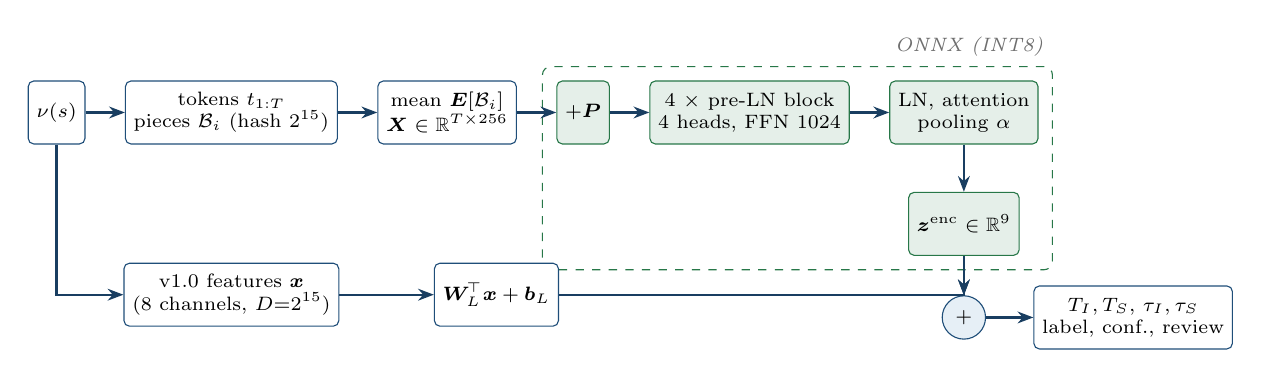
\begin{tikzpicture}[
  node distance=0.35cm and 0.5cm,
  box/.style={draw=accent,rounded corners=2pt,fill=accentlight!60,minimum height=0.8cm,align=center,font=\scriptsize,inner sep=3pt},
  np/.style={box,fill=white},
  onnx/.style={box,fill=okgreen!12,draw=okgreen},
  arr/.style={-{Stealth[length=2mm]},thick,accent!80!black},
  lab/.style={font=\scriptsize\itshape,text=muted}]
  \node[np] (txt) {$\nu(s)$};
  \node[np,right=of txt] (tok) {tokens $t_{1:T}$\\pieces $\mathcal{B}_i$ (hash $2^{15}$)};
  \node[np,right=of tok] (emb) {mean $\bm E[\mathcal{B}_i]$\\$\bm X\in\R^{T\times256}$};
  \node[onnx,right=of emb] (pos) {$+\bm P$};
  \node[onnx,right=of pos] (blk) {4 $\times$ pre-LN block\\4 heads, FFN 1024};
  \node[onnx,right=of blk] (pool) {LN, attention\\pooling $\alpha$};
  \node[onnx,below=0.6cm of pool] (head) {$\z^{\text{enc}}\in\R^9$};
  \node[np,below=1.5cm of tok] (feat) {v1.0 features $\x$\\(8 channels, $D{=}2^{15}$)};
  \node[np,right=1.2cm of feat] (lin) {$\W_L^{\!\top}\x+\bb_L$};
  \node[box,circle,inner sep=1pt,minimum height=0.55cm,below=0.5cm of head] (plus) {$+$};
  \node[np,right=0.6cm of plus] (cal) {$T_I,T_S$, $\tau_I,\tau_S$\\label, conf., review};
  \draw[arr] (txt) -- (tok);
  \draw[arr] (tok) -- (emb);
  \draw[arr] (emb) -- (pos);
  \draw[arr] (pos) -- (blk);
  \draw[arr] (blk) -- (pool);
  \draw[arr] (pool) -- (head);
  \draw[arr] (txt) |- (feat);
  \draw[arr] (feat) -- (lin);
  \draw[arr] (lin) -| (plus);
  \draw[arr] (head) -- (plus);
  \draw[arr] (plus) -- (cal);
  \begin{scope}[on background layer]
    \node[draw=okgreen,dashed,rounded corners=3pt,fit=(pos)(blk)(pool)(head),inner sep=5pt,
          label={[lab,anchor=south east]north east:ONNX (INT8)}] {};
  \end{scope}
\end{tikzpicture}
\caption{Student at inference. White boxes run in NumPy (hashing, embedding mean, linear branch, calibration); the green region is the exported ONNX encoder.}
\label{fig:student}
\end{figure}

\begin{table}[h]
\centering\small
\caption{Parameter breakdown and comparison with the v1.1 attention branch.}
\label{tab:params}
\begin{tabular}{@{}l r r@{}}
\toprule
Component & v1.1 & v1.2 student \\
\midrule
Piece embeddings & $2^{14}\times32 = 524{,}288$ & $2^{15}\times256 = 8{,}388{,}608$ \\
Positions & $128\times32 = 4{,}096$ & $128\times256 = 32{,}768$ \\
Contextual layers & 1 single-head attention: 4{,}096 & 4 pre-LN blocks: 3{,}159{,}040 \\
Pooling $+$ output & $32 + 288 = 320$ & 3{,}082 \\
Hashed linear branch & 294{,}921 & 294{,}921 \\
\midrule
\textbf{Total} & \textbf{827{,}721} & \textbf{11{,}878{,}419} \\
Without linear branch & 532{,}800 & 11{,}583{,}498 \\
\bottomrule
\end{tabular}
\end{table}

\begin{table}[h]
\centering\small
\caption{Architectural differences at a glance.}
\label{tab:archdiff}
\begin{tabularx}{\linewidth}{@{}l X X@{}}
\toprule
& v1.1 attention branch & v1.2 student \\
\midrule
Token representation & mean of hashed pieces, $B=2^{14}$, $d=32$ & same pieces, $B=2^{15}$, $d=256$ \\
Context & 1 layer, 1 head, residual $\tanh$, no FFN, no LayerNorm & 4 pre-LN layers, 4 heads, GELU FFN 1024 \\
Pooling & $\softmax(\bm H\bm u)$ & $\softmax(\bm H\bm w_\alpha + b_\alpha)$ with padding mask \\
Lexical branch & v1.0 linear, logits added & identical \\
Training signal & gold labels only & gold $+$ teacher soft labels $+$ consistency \\
Optimizer & per-example Adam $+$ sparse Adagrad (NumPy) & AdamW, cosine, fp16, batch 64 (PyTorch) \\
Runtime & NumPy & NumPy $+$ ONNX Runtime INT8 \\
\bottomrule
\end{tabularx}
\end{table}

\subsection{Objective}
With student logits $\z$, teacher logits $\z_{\text{T}}$, gold-label masks $\mu$, KD masks $\kappa$ and a meaning-preserving noisy copy $\tilde s$:
\begin{align}
  \mathcal{L}_{\text{CE}} &= \sum_{k} \frac{1}{\sum_i\mu^k_i}\sum_i \mu^k_i\,\alpha^k_{y^k_i}\,\CE\big(\softmax(\z^k_i), y^k_i\big), \\
  \mathcal{L}_{\text{KD}} &= \sum_{k} \frac{1}{\sum_i\kappa^k_i}\sum_i \kappa^k_i\; \tau^2\,\KL\Big(\softmax(\z^k_{\text{T},i}/\tau)\,\Big\|\,\softmax(\z^k_i/\tau)\Big),\qquad \tau = 2, \\
  \mathcal{L}_{\text{cons}} &= \frac{1}{N}\sum_i\sum_k \KL\Big(\mathrm{sg}\big[\softmax(\z^k(s_i))\big]\,\Big\|\,\softmax(\z^k(\tilde s_i))\Big), \\
  \mathcal{L} &= \mathcal{L}_{\text{CE}} + \lambda_{\text{KD}}\,\mathcal{L}_{\text{KD}} + \lambda_{\text{cons}}\,\mathcal{L}_{\text{cons}},\qquad \lambda_{\text{KD}}=1,\ \lambda_{\text{cons}}=0.1 .
\end{align}
$\mathrm{sg}$ is stop-gradient. $\tilde s$ uses only character noise on editable tokens (never negators, emoji or punctuation, never a stress-map output), so consistency is not imposed across meaning-changing edits.

\paragraph{Epoch composition.} All 4{,}061 support rows every epoch; 4{,}000 public labeled tweets and 8{,}000 pool sentences re-sampled each epoch with a generator seeded by $1000\cdot\text{seed}+e$ (16{,}061 rows, 251 steps at batch 64). Token dropout removes whole tokens with $p=0.15$ (at least one kept).

\paragraph{Variants (notebook 03, in order).} Student $+$ KD (seed 42); student without KD on identical labeled data (pool rows drop out automatically); student $+$ KD without the linear branch; seeds 43 and 44 if the 100-minute guard allows.

\paragraph{Training outcome.} All five variants finished (one Colab disconnect, resumed automatically). Best validation NLL: 0.0647 (KD, s42, epoch 10), 0.1483 (no-KD), 0.1483 (no linear branch), 0.1558 (s43), 0.1018 (s44); 16{,}061 rows per epoch took $\sim$42\,s on a T4.

\paragraph{Pipeline check (not a result).} One CPU epoch of the real configuration on the real KD files hashes 66{,}166 rows in 36.5\,s and reaches validation NLL 0.537 (v1.1 after calibration: 0.469); it verifies the pipeline only.

% ============================================================================
\section{Deployment Runtime}
\label{sec:deploy}

The trained student is split at the boundary between sparse lookups and dense computation:
\begin{enumerate}
  \item \texttt{embeddings.npz}: $\bm E$, $\W_L$, $\bb_L$ (NumPy; \texttt{np.add.reduceat} computes \cref{eq:embed});
  \item \texttt{encoder.onnx}: positions, 4 blocks, pooling and head; inputs $\bm X\in\R^{1\times T\times256}$ and mask, outputs $\z^{\text{enc}}$ and $\bm\alpha$; opset 17 with a dynamic token axis;
  \item \texttt{encoder.int8.onnx}: ONNX Runtime dynamic quantization (INT8 weights, dynamic activation scales);
  \item \texttt{meta.json}: configuration and calibration fitted on the \emph{deployed INT8 model's} validation logits with the v1.1 algorithm.
\end{enumerate}
Torch-vs-ONNX parity (fp32) is $6.7\times10^{-7}$ maximum absolute logit difference over all evaluation messages. An exporter pitfall was found and fixed: exporting through a wrapper module re-enables training mode recursively afterwards, which silently switched dropout on for the parity check (difference 0.29 before the fix). \texttt{python v12/predict.py "text"} returns the v1.1 JSON (\lbl{label}, \lbl{confidence}, \lbl{review\_required} per head), optionally with $\bm\alpha$.

\subsection{Latency (architecture measurement)}
Apple M2, Python 3.12, NumPy 2.3.5, ONNX Runtime 1.30; 80 warm-up and 600 timed calls at batch 1, including hashing, embedding mean, encoder, linear branch, calibration and JSON serialization (whitepaper protocol). All numbers below are for the trained student (\texttt{results/latency\_student\_kd\_s42.json}); ONNX FP32 parity with PyTorch is $5.8\times10^{-6}$ and INT8 changes 1 of 190 test sentiment predictions and no intent prediction.

\begin{table}[h]
\centering\small
\caption{Latency by precision and ONNX Runtime intra-op threads (ms).}
\label{tab:latency}
\begin{tabular}{@{}l ccc c@{}}
\toprule
Configuration & p50 & p95 & p99 & 512 code points, p95 \\
\midrule
INT8, 1 thread  & 0.64 & 0.92 & 1.15 & 5.98 \\
\textbf{INT8, 2 threads} & \textbf{0.57} & \textbf{0.81} & \textbf{0.90} & \textbf{4.29} \\
INT8, 4 threads & 0.53 & 0.77 & 0.95 & 3.45 \\
FP32, 1 thread  & 1.14 & 1.62 & 1.75 & 10.96 \\
FP32, 2 threads & 0.81 & 1.14 & 1.23 & 6.83 \\
FP32, 4 threads & 0.68 & 1.00 & 1.39 & 4.91 \\
\midrule
v1.1, same machine & 0.27 & 0.38 & 0.45 & 1.40 \\
\bottomrule
\end{tabular}
\end{table}

\begin{table}[h]
\centering\small
\caption{Worst case (512 code points, 106 tokens, 920 pieces): an earlier architecture-only sweep over threads (600 calls each, untrained weights) and cost breakdown at 1 thread.}
\label{tab:sweep}
\begin{tabular}{@{}l ccc@{}}
\toprule
INT8 threads & p50 & p95 & p99 \\
\midrule
1 & 5.74 & 6.11 & 7.38 \\
\textbf{2} & \textbf{4.05} & \textbf{4.53} & 6.26 \\
3 & 3.45 & 4.44 & 7.09 \\
4 & 3.10 & 5.10 & 7.13 \\
\bottomrule
\end{tabular}
\hspace{1.5em}
\begin{tabular}{@{}l r@{}}
\toprule
Stage (1 thread) & ms \\
\midrule
token pieces (hashing) & 0.30 \\
v1.0 features (hashing) & 0.80 \\
embedding mean & 0.30 \\
ONNX encoder (INT8) & 4.32 \\
linear branch & 0.004 \\
\midrule
full predict & 6.03 \\
\bottomrule
\end{tabular}
\end{table}

Typical messages are about six times inside the 5\,ms budget. The worst case is dominated by the encoder; two threads keep p95 below 5\,ms (4.29\,ms trained, 4.53\,ms in the earlier sweep), while four threads were noisy on the M2's mixed performance/efficiency cores (3.45, 3.84 and 5.10\,ms across three measurements). p99 at 512 code points exceeded 5\,ms in the sweep. \texttt{predict.py} defaults to 2 threads. v1.1 remains 2--3$\times$ faster.

% ============================================================================
\section{Results So Far}
\label{sec:results}

\begin{table}[t]
\centering\small
\caption{Development test (190 rows, 44 groups): macro-F1 with 95\% group-bootstrap interval and paired difference vs v1.1 on identical resamples.}
\label{tab:main}
\setlength{\tabcolsep}{3.5pt}
\resizebox{\linewidth}{!}{%
\begin{tabular}{@{}l r cc cc c cc c c@{}}
\toprule
& & \multicolumn{2}{c}{Intent} & \multicolumn{2}{c}{Sentiment} & Pos. & \multicolumn{2}{c}{Stress F1 (consist.)} & Emoji & Audit \\
\cmidrule(lr){3-4}\cmidrule(lr){5-6}\cmidrule(lr){8-9}
System & Params & F1 [95\% CI] & $\Delta$ vs v1.1 & F1 [95\% CI] & $\Delta$ vs v1.1 & recall & Intent & Sent. & pairs & err. \\
\midrule
v1.1 full & 0.83M & .901 [.78, .97] & -- & .845 [.72, .94] & -- & .72 & .865 (97.4\%) & .826 (92.6\%) & 9/12 & 6 \\
Teacher (v1.1 data) & 278M & .929 [.82, 1.00] & $+.032$ [$-.06$, $+.14$] & 1.000 [1.00, 1.00] & $\mathbf{+.159}$ [$+.06$, $+.28$] & 1.00 & .852 (92.6\%) & 1.000 (100\%) & 12/12 & 1 \\
Teacher v2 & 278M & \textbf{.966} [.92, .99] & $+.071$ [$-.007$, $+.172$] & 1.000 [1.00, 1.00] & $\mathbf{+.159}$ [$+.06$, $+.28$] & 1.00 & \textbf{.933} (95.8\%) & 1.000 (100\%) & 12/12 & 1 \\
\midrule
Student $+$ KD (s42) & 11.88M & .914 [.81, .98] & $+.014$ [$-.10$, $+.13$] & .911 [.82, .98] & $+.068$ [$-.07$, $+.21$] & 1.00 & .914 (97.9\%) & .917 (96.3\%) & 12/12 & 2 \\
Student no-KD (s42) & 11.88M & .888 [.77, .97] & $-.011$ [$-.12$, $+.11$] & .878 [.77, .96] & $+.034$ [$-.07$, $+.14$] & .93 & .895 (96.8\%) & .836 (92.6\%) & 12/12 & 3 \\
Student $+$ KD w/o linear (s42) & 11.58M & .958 [.89, .99] & $+.062$ [$-.03$, $+.17$] & .909 [.81, .98] & $+.066$ [$-.04$, $+.17$] & .93 & .918 (94.7\%) & .925 (96.3\%) & 11/12 & 1 \\
Student $+$ KD (s43) & 11.88M & .911 [.82, .98] & $+.014$ [$-.09$, $+.14$] & .853 [.74, .94] & $+.009$ [$-.11$, $+.13$] & .95 & .910 (98.9\%) & .813 (88.9\%) & 12/12 & 3 \\
Student $+$ KD (s44) & 11.88M & .919 [.82, .98] & $+.020$ [$-.09$, $+.13$] & .952 [.87, 1.00] & $+.110$ [$-.00$, $+.23$] & .93 & .914 (97.9\%) & .925 (97.4\%) & 12/12 & 1 \\
\textbf{Student $+$ KD, ONNX INT8} & 11.88M & .914 [.81, .98] & $+.014$ [$-.10$, $+.13$] & .916 [.83, .98] & $+.073$ [$-.06$, $+.22$] & 1.00 & .914 (97.9\%) & .917 (95.8\%) & 12/12 & 2 \\
\bottomrule
\end{tabular}}
\end{table}

\begin{table}[h]
\centering\small
\caption{Calibration and selective prediction on test (temperature and review threshold fitted on validation).}
\label{tab:calib}
\begin{tabular}{@{}l cc cc cc cc@{}}
\toprule
& \multicolumn{2}{c}{Temperature} & \multicolumn{2}{c}{ECE} & \multicolumn{2}{c}{Coverage} & \multicolumn{2}{c}{Acc.\ on accepted} \\
\cmidrule(lr){2-3}\cmidrule(lr){4-5}\cmidrule(lr){6-7}\cmidrule(lr){8-9}
System & $T_I$ & $T_S$ & int & sent & int & sent & int & sent \\
\midrule
v1.1 & 0.550 & 1.316 & .082 & .106 & .953 & .753 & .906 & .951 \\
Teacher (v1.1 data) & 0.595 & 1.316 & .070 & .014 & 1.000 & 1.000 & .916 & 1.000 \\
Teacher v2 & 0.400$^\ast$ & 0.508 & .044 & .000 & 1.000 & 1.000 & .963 & 1.000 \\
Student $+$ KD (s42) & 0.400$^\ast$ & 0.755 & .070 & .048 & 1.000 & 1.000 & .921 & .911 \\
Student $+$ KD, INT8 & 0.400$^\ast$ & 0.755 & .070 & .045 & 1.000 & 1.000 & .921 & .916 \\
\bottomrule
\end{tabular}
\\[2pt]{\footnotesize $^\ast$ lower boundary of the temperature grid.}
\end{table}

\begin{table}[h]
\centering\small
\caption{Data ablation: teacher v2 minus Phase~1 teacher (same encoder, same selection rule, different training data).}
\label{tab:ablation}
\begin{tabular}{@{}l c c c@{}}
\toprule
Head & Mean $\Delta$ & 95\% CI & $P(\Delta>0)$ \\
\midrule
Intent & $+0.040$ & $[-0.028, +0.121]$ & 0.85 \\
Sentiment & $0.000$ & $[0.000, 0.000]$ & -- (both at ceiling) \\
\bottomrule
\end{tabular}
\end{table}

\begin{table}[h]
\centering\small
\caption{Student ablations and distillation gap: paired differences on the same 5{,}000 resamples.}
\label{tab:studentpaired}
\begin{tabular}{@{}l cc cc@{}}
\toprule
& \multicolumn{2}{c}{Intent} & \multicolumn{2}{c}{Sentiment} \\
\cmidrule(lr){2-3}\cmidrule(lr){4-5}
Comparison & $\overline\Delta$ [95\% CI] & $P(\Delta>0)$ & $\overline\Delta$ [95\% CI] & $P(\Delta>0)$ \\
\midrule
KD effect: student $+$ KD $-$ no-KD (s42) & $+0.025$ [$-0.034$, $+0.113$] & 0.70 & $+0.034$ [$-0.055$, $+0.124$] & 0.78 \\
Linear branch: with $-$ without (s42) & $-0.048$ [$-0.124$, $+0.014$] & 0.07 & $+0.002$ [$-0.091$, $+0.094$] & 0.51 \\
Student $+$ KD $-$ teacher v2 & $-0.057$ [$-0.136$, $+0.004$] & 0.04 & $\mathbf{-0.092}$ [$-0.184$, $-0.020$] & 0.00 \\
INT8 $-$ FP32 (s42) & $+0.000$ [$+0.000$, $+0.000$] & -- & $+0.005$ [$+0.000$, $+0.017$] & 0.64 \\
\bottomrule
\end{tabular}
\\[2pt]{\footnotesize Seed spread of student $+$ KD (seeds 42/43/44): intent mean 0.915, sd 0.004; sentiment mean 0.906, sd 0.049. Best validation NLL ranged from 0.065 (s42) to 0.156 (s43).}
\end{table}

\paragraph{Reading the students.} (i) \emph{Distillation gap:} the student is significantly below teacher~v2 on sentiment and trends below on intent; the KD soft labels do not transfer the teacher's sentiment robustness. (ii) \emph{KD effect:} positive point estimates, unresolved, and smaller than the seed standard deviation of the primary variant; the no-KD student even solves one more contrast pair. (iii) \emph{Linear branch:} removing it improves intent (0.958, 20/40 contrast pairs) with $P(\Delta>0)=0.07$ for keeping it; the deployed model keeps the branch because it was the pre-specified primary variant, and a single seed does not justify switching. (iv) \emph{Stability:} unseen-misspelling consistency is at least v1.1's level (97.9\% vs 97.4\%) and emoji pairs are 12/12, but negated negatives stay at 1/10 pairs for every student and seed~43 reintroduces the \hi{cancel mat karna} audit error. (v) \emph{Calibration:} validation thresholds collapse to 0, so the student never defers to review on this split (v1.1 sentiment coverage was 0.753).

% ============================================================================
\section{Discussion}
\label{sec:discussion}

\subsection{What Improved and What Did Not}
\begin{itemize}
  \item \textcolor{okgreen}{\textbf{Improved}}: sentiment on every set; positive recall; emoji contrast pairs (RoBERTa tokenizers); the \hi{nahi}$\Rightarrow$\lbl{negative} cue; audit errors (6$\to$1); negation-scope intent on the contrast set (0.65$\to$0.90, teacher~v2); robustness to unseen misspellings (stress intent 0.865$\to$0.933, teacher~v2).
  \item \textcolor{warn}{\textbf{Not resolved}}: intent gains over v1.1 and over the Phase~1 teacher on 44 test groups (all CIs include 0); keyword routing of \hi{\dots nahi mila} to \lbl{not\_received}; feedback about logistics routed to operational intents; negated negatives remain at 6/10 pairs for both teachers.
  \item \textcolor{okgreen}{\textbf{Student, improved}}: a deployable 11.88M-parameter model at 0.81\,ms p95; INT8 lossless; stress consistency 97.9\%; emoji pairs 12/12; positive recall 1.00; 17/40 contrast pairs vs 10/40 for v1.1.
  \item \textcolor{warn}{\textbf{Student, not achieved}}: gains over v1.1 are not resolved on either head; sentiment is significantly below teacher~v2; KD not shown to help; the linear branch appears to hurt intent; negated negatives 1/10 pairs; sentiment unstable across seeds; review flag never fires.
\end{itemize}

\subsection{Threats to Validity}
\begin{itemize}
  \item \textbf{Same generator.} v1.1 test and audit, most training data, the generated messages and the contrast set were written by LLMs (the last two by the same assistant). Gains may partly reflect matching the generator's style; generated data lifts validation/test vocabulary coverage to $\sim$0.94. Sentiment 1.000 is a ceiling on this distribution.
  \item \textbf{Contrast vocabulary overlap.} 18 contrast affect words enter training via generated data; UA results after Phase~2 are not generalisation evidence.
  \item \textbf{Out-of-domain public data.} Political, cricket, movie and chit-chat tweets with visible label noise (teacher--gold agreement 0.71), restrictive licenses.
  \item \textbf{Pseudo-label noise.} Sentiment soft labels on 50{,}000 unlabeled tweets come from a teacher trained on 4{,}000 of them plus support data.
  \item \textbf{Seeds and power.} One seed per teacher; three student seeds only for the primary variant, while the KD and linear-branch ablations use one seed and are smaller than the primary variant's sentiment sd (0.049); 44 test groups.
  \item \textbf{Free-GPU training.} Colab T4; teacher checkpoints omit optimizer moments; $\le$3 learning rates; public-only pre-fine-tuning stage skipped.
  \item \textbf{No human data.} No real customer messages; the evaluator scores \texttt{data/human\_test.jsonl} separately if it is added.
\end{itemize}

\subsection{Requirements Scorecard (interim)}
\begin{table}[h]
\centering\small
\caption{Status against the v1.2 constraints.}
\label{tab:scorecard}
\begin{tabularx}{\linewidth}{@{}l l X@{}}
\toprule
Requirement & Status & Evidence \\
\midrule
Student $\le$15M parameters & \textcolor{okgreen}{\textbf{Met}} & 11{,}878{,}419 (\cref{tab:params}) \\
p95 $<5$\,ms, batch 1, Mac CPU, incl.\ hashing & \textcolor{okgreen}{\textbf{Met}} (2 threads) & 0.81\,ms on test messages; 4.29\,ms at 512 code points with 2 threads; 5.98\,ms with 1 thread (\cref{tab:latency}) \\
Exact v1.1 splits, validation-only choices & \textcolor{okgreen}{\textbf{Met}} & digest-checked export; \cref{sec:protocol} \\
Near-duplicate filtering & \textcolor{okgreen}{\textbf{Met}} & removed: public 0, generated 1, augmented 2 \\
Hash parity Colab $\leftrightarrow$ Mac & \textcolor{okgreen}{\textbf{Met}} & 50/50 fixtures; Python 3.10--3.14 \\
Sentiment robustness & \textcolor{pending}{\textbf{Teachers only}} & teachers $+0.159$ $[+0.056, +0.282]$; student $+0.068$ $[-0.07, +0.21]$, seed sd 0.049 \\
Distillation keeps teacher gains & \textcolor{warn}{\textbf{Not met}} & student $-$ teacher~v2 sentiment $-0.092$ $[-0.184, -0.020]$ (\cref{tab:studentpaired}) \\
Negation scope & \textcolor{pending}{\textbf{Partial}} & teacher~v2: NS intent 0.90, 6/10 pairs; deployed student 5/10 pairs \\
Real-world validation & \textcolor{warn}{\textbf{Not met}} & no human-collected data \\
\bottomrule
\end{tabularx}
\end{table}

% ============================================================================
\appendix
\section{Hyperparameters}
\begin{table}[h]
\centering\small
\begin{tabular}{@{}l l l@{}}
\toprule
Setting & Teacher (01 / 02) & Student (03) \\
\midrule
Encoder & 4 candidates / hing-roberta-mixed & 4 pre-LN blocks, $d{=}256$, 4 heads, FFN 1024 \\
Learning rates & \{2,3,5\}e-5 / \{3,5\}e-5 & 5e-4 (AdamW) \\
Batch, max length & 16 / 32; 128 subwords & 64; 128 tokens \\
Schedule & 10\% / 6\% warm-up, linear decay & 5\% warm-up, cosine \\
Epochs, patience & 12, 3 / 6, 2 & 30, 5 \\
Regularization & dropout 0.1, weight decay 0.01, clip 1.0 & dropout 0.1, token dropout 0.15, weight decay 0.01, clip 1.0 \\
Loss weights & class-balanced CE & CE $+$ 1.0 KD ($\tau{=}2$) $+$ 0.1 consistency \\
Precision & fp16 autocast & fp16 autocast \\
Hash buckets & -- & pieces $2^{15}$; linear $2^{15}$ \\
Seed & 42 & 42 (43, 44) \\
Selection & min.\ validation NLL & min.\ validation NLL \\
\bottomrule
\end{tabular}
\end{table}

\section{Reproduction}
\begin{lstlisting}
uv venv --python 3.12 .venv-v12
uv pip install --python .venv-v12/bin/python -r v12/requirements-v12.txt
cd v12
make smoke          # CPU smoke test of every trainer (disconnect + resume)
make bundle         # notebooks + bundle.zip for Colab/Kaggle
# Colab T4: notebooks/01_teacher -> 02_teacher_kd -> 03_student ("Run all")
unzip -o 01_teacher_outputs.zip -d runs/01_teacher && make eval-teacher
unzip -o 02_teacher_kd_outputs.zip -d runs/02_teacher_kd && make teacher-v2
unzip -o 03_student_outputs.zip -d runs/03_student && make deploy
make compare        # results/phase5_table.md
python predict.py "cancel mat karna, bas track karo"
\end{lstlisting}

\section{Notebooks}
\begin{table}[h]
\centering\small
\begin{tabular}{@{}l l r l@{}}
\toprule
Notebook & Content & GPU time & Status \\
\midrule
01\_teacher & 4 encoders $\times$ 3 LR, v1.1 train & 38.4 min (T4) & done \\
02\_teacher\_kd & teacher v2 $+$ logits for 66{,}166 KD rows & 10.2 min (T4) & done \\
03\_student & 5 student variants (1 disconnect, resumed) & $\sim$45 min (T4) & done \\
\bottomrule
\end{tabular}
\end{table}

\section{Emoji Notation}
\emo{unamused} = U+1F612, \emo{smile} = U+1F60A, \emo{angry} = U+1F621 / U+1F620, \emo{huff} = U+1F624, \emo{thumbs-up} = U+1F44D. The system operates on the actual code points.

\end{document}
